% The loss plot in examples/tikz-demo.tex. Compile with pdflatex, then make the PNG the editor
% shows: pdftoppm -png -r 200 -singlefile loss.pdf loss
\documentclass[border=6pt]{standalone}
\usepackage{pgfplots}
\pgfplotsset{compat=1.18}
\begin{document}
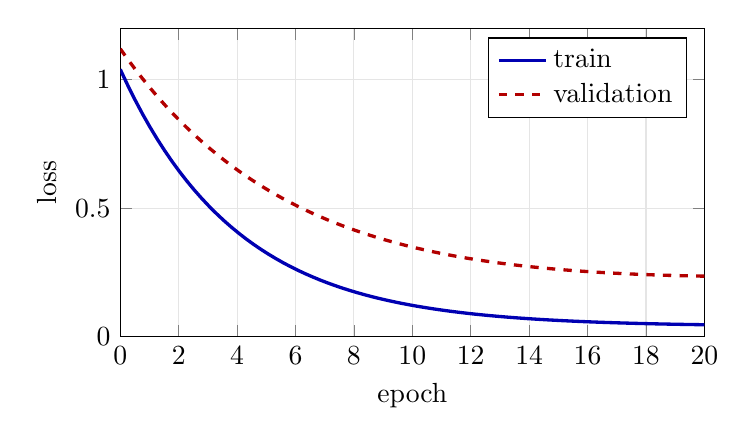
\begin{tikzpicture}
  \begin{axis}[
      width=9cm, height=5.5cm,
      xlabel={epoch}, ylabel={loss},
      xmin=0, xmax=20, ymin=0, ymax=1.2,
      grid=major, grid style={gray!20},
      legend pos=north east, legend cell align=left
    ]
    \addplot[blue!70!black, very thick, domain=0:20, samples=80] {exp(-x/4) + 0.04};
    \addplot[red!70!black, very thick, dashed, domain=0:20, samples=80] {exp(-x/6) + 0.12 + 0.004*x};
    \legend{train, validation}
  \end{axis}
\end{tikzpicture}
\end{document}
